\documentclass[11pt]{article}
\usepackage{amsmath,amssymb}
\usepackage{natbib}
\usepackage[hmargin=2cm,vmargin=4cm]{geometry}
\usepackage{color}
\usepackage{graphicx,wrapfig,lipsum}

\usepackage{titling}

\setlength{\droptitle}{-11em}   % This is your set screw

\title{Energy Disaggregation using Non-Intrusive Load Monitoring}

\author{Karen Yu, Nick Vasios and Thibaut Perol\\ \small Final project for AM207}
\date{}
\begin{document}
\maketitle


\section{Abstract}

\section{Introduction}

Energy disaggregation is the procedure that infers the energy consumption in the basis of appliances in a household given the total energy consumption from a single meter of that household. In recent years, this field has become increasingly popular as smart meters have begun to deploy and are installed in many households across the world. However, the field's popularity is mostly attributed to the extremely powerful techniques which are able to take advantage of the continuously improving computational resources and perform this disaggregation in a non-intrusive manner. The term non-intrusive implies that the appliance-based energy consumption is not determined by installing individual meters on each appliance and thus interfering with the occupant's privacy, but rather by estimating it using both deterministic and stochastic techniques.
\begin{figure}
\begin{center}
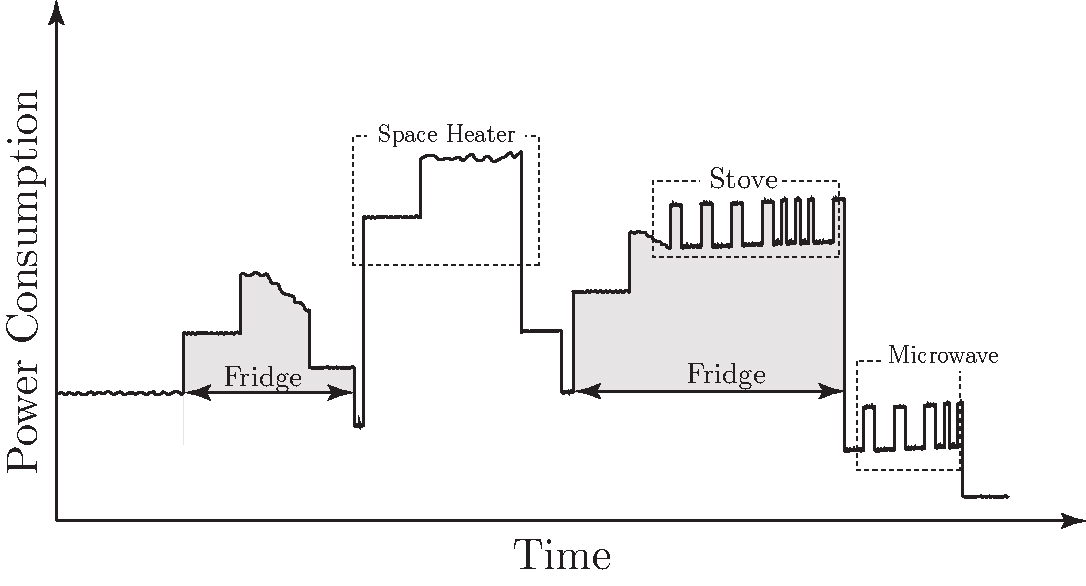
\includegraphics[width= 20 pc]{./../poster/Figures/Qualitative}
\caption*{\footnotesize  \textbf{Figure}: Typical Power Consumption in a household within a time frame that many appliances activate and deactivate} \vspace*{-1 cm}
\end{center}
\end{figure}

\section{Methods}

\section{Results}

\section{Conclusion}



\bibliographystyle{agufull08}
\bibliography{/Users/thibaut/Dropbox/Biblio/Perol_biblio}

\end{document}
